\documentclass[xetex]{beamer}
\usepackage{fontspec}
\usepackage{bytefield}

\title{Automatisk upptäckt av strukturer för binära nätverksprotokoll}
\author{Fredrik Appelros \& Carl Ekerot}
\date

% Introducera problemet - applikationer
% Tidigare försök
% Kort om vårt angreppssätt
% Hitta pakettyper (2 delar)
% Klustring
% Förfining av typindelning
% Fältanalys (bygger på bytefördelningar)
% Olika fälttyper
% Tillståndsdiagram
% Resultat - jämförelse mellan definition och inferens
% Begränsningar

\begin{document}
    \frame{\titlepage}
    
    % Introduktion
    \begin{frame}
        \frametitle{Binära nätveksprotokoll}
        \begin{columns}[t]
            \begin{column}[T]{8cm}
                \begin{itemize}
                    \item Språk för mjukvara eller hårdvara
                    \item Binärt kodat -- ej läsbart
                    \item Läses med hjälp av specifikation
                    \item Byggs upp av fält som representerar nummer, flaggor,
                        data osv.
                    \item Exempel: DNS, SMB, RTP, DHCP, \ldots
                \end{itemize}
            \end{column}
            \begin{column}[T]{6cm}
                \begin{bytefield}[bitwidth=0.56em]{16}
                    \bitheader{0, 16}\\
                    \wordbox{1}{\texttt{1000011010010000}}\\
                    \bitbox{1}{\texttt{1}}
                    \bitbox{4}{\texttt{0000}}
                    \bitbox{1}{\texttt{0}}
                    \bitbox{1}{\texttt{0}}
                    \bitbox{1}{\texttt{1}}
                    \bitbox{1}{\texttt{1}}
                    \bitbox{3}{\texttt{000}}
                    \bitbox{4}{\texttt{0000}}\\
                    \wordbox{1}{\texttt{0000000000000001}}\\
                    \wordbox{1}{\texttt{0000000000000010}}\\
                    \wordbox{1}{\texttt{0000000000000001}}\\
                    \wordbox{1}{\texttt{0000000000000000}}
                \end{bytefield}
            \end{column}
        \end{columns}
    \end{frame}
    \begin{frame}
        \frametitle{Slutna protokoll}
        \begin{itemize}
            \item Ett protokoll kan ha \emph{öppen} eller \emph{sluten}
                specifikation
            \item Slutet protokoll $\Rightarrow$ svårt att tyda meddelanden
            \item Proprietära eller odokumenterade
            \item Exempel: Skype, (tidigare) SMB
        \end{itemize}
        \vskip20pt
        Varför avkoda slutna protokoll?
        \begin{enumerate}
            \item Interoperabilitet (SMB)
            \item QoS
        \end{enumerate}
    \end{frame}
    \begin{frame}
        \frametitle{Tidigare försök}
        Discoverer, Microsoft (2005)
        \begin{itemize}
            \item Arbetar på lagrad nätverkstrafik
            \item Delar upp i textuell och binär data
            \item Försöker hitta meddelandetyper
        \end{itemize}
        \vskip20pt
        Dispatcher, UC Berkeley (2012)
        \begin{itemize}
            \item Övervakar exekveringstillstånd
            \item Jämför nätverkstrafik med data i minnet
            \item Kräver mjukvaran/hårdvaran som använder protokollet
        \end{itemize}
    \end{frame}

    % Vår approach
    \begin{frame}
        \frametitle{Vårt angreppssätt}
        Input: Nätverksdump (pcap)\\
        Metod:
        \begin{enumerate}
            \item Identifiera meddelandetyper
                \begin{itemize}
                    \item Statistisk analys -- \emph{klustring}
                    \item Förfining -- hitta vad som definierar en meddelandetyp
                \end{itemize}
            \item Identifiera fält
                \begin{itemize}
                    \item Statistisk analys -- identifiera bytevärdesdistributioner
                    \item Identifiera fält specifika för anslutningar
                    \item Hitta längdfält
                \end{itemize}
            \item Bygg tillståndsdiagram
                \begin{itemize}
                    \item Vilka meddelandetyper kan följa ett visst meddelande?
                \end{itemize}
        \end{enumerate}
    \end{frame}
    
    % Klustring
    \begin{frame}
        \frametitle{Hitta meddelandetyper}
        \begin{itemize}
            \item Antagande: liknande data $\Leftrightarrow$ samma meddelandetyp
            \item Klustring: gruppera datapunkter m.a.p. egendefinierade egenskaper
                för varje datapunkt
            \item Använda resultat från klustring för att hitta de bytes som
                definierar ett meddelandes typ
        \end{itemize}
    \end{frame}
    \begin{frame}
        \frametitle{Hitta meddelandetyper -- Klustring}
        Problem:
        \begin{itemize}
            \item Okänt antal kluster (meddelandetyper)
            \item Varierande \emph{täthet} bland kluster
        \end{itemize}
        Lösning: \textbf{OPTICS}, \scriptsize{
            \emph{\underline{O}rdering \underline{P}oints \underline{T}o
                  \underline{I}dentify the \underline{C}lustering 
                  \underline{S}tructure}}
        \vskip20pt
        \begin{columns}[t]
            \begin{column}[T]{6cm}
                \begin{itemize}
                    \item \emph{Densitetsbaserad} klustringsalgoritm
                    \item Hittar kluster med olika täthet
                    \item Behöver ej fördefinierat antal kluster som parameter
                \end{itemize}
            \end{column}
            \begin{column}[T]{6cm}
                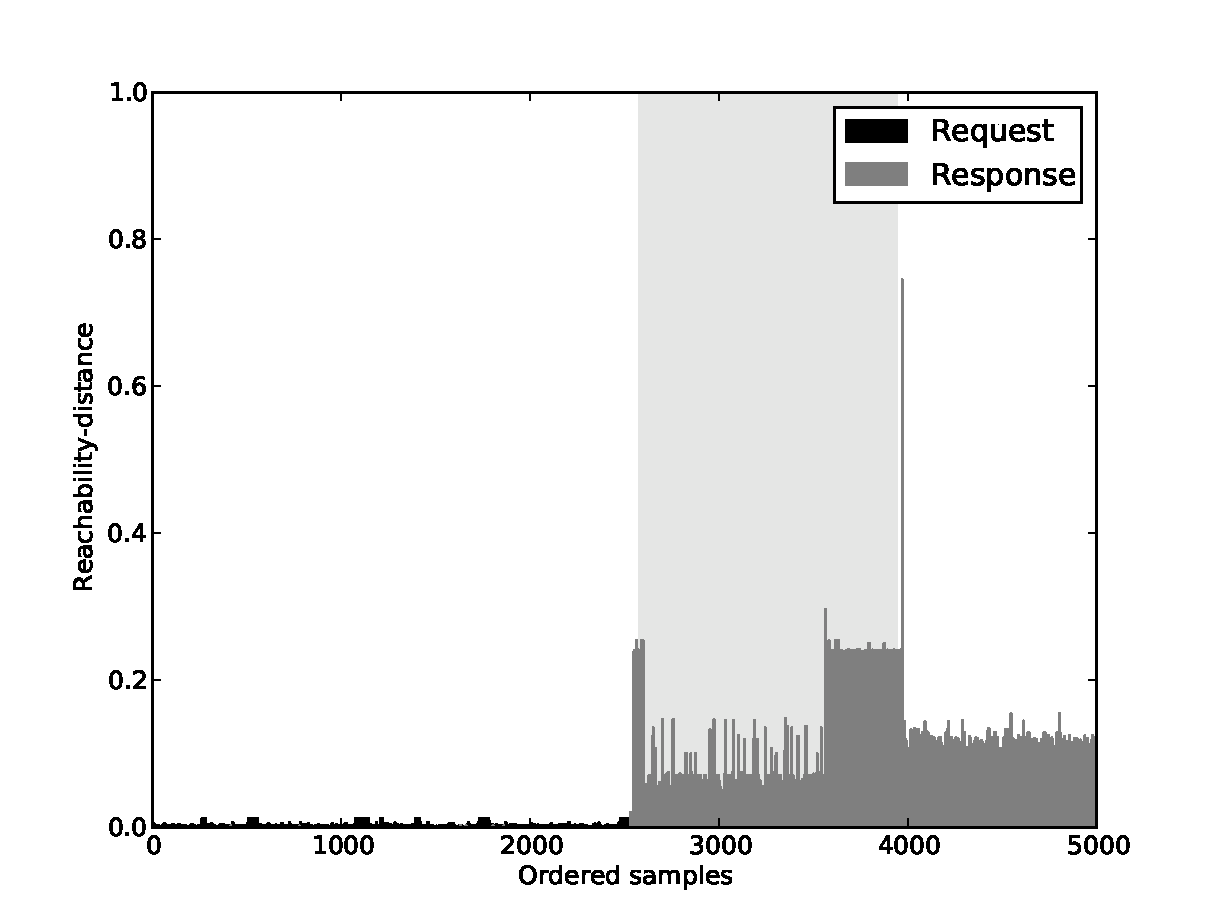
\includegraphics[height=4.5cm]{img/hierextr.pdf}
            \end{column}
        \end{columns}
    \end{frame}
    \begin{frame}
        \frametitle{Hitta meddelandetyper -- Klustring (forts.)}
        Egenskaper: vektor $\{f_1, f_2, ..., f_n\}$
        \begin{itemize}
            \item $n$: meddelandets längd
            \item $f_i$: sannolikhet för att bytevärdet på position $i$ i
                meddelandet är det värdet som det är.
        \end{itemize}
        \vskip20pt
        Problem: hög dimensionalitet \\
        Lösning: \textbf{PCA}, \scriptsize{\underline{P}rincipal
            \underline{C}omponent \underline{A}nalysis}
    \end{frame}
    \begin{frame}
        \frametitle{Hitta meddelandetyper -- Förfining}
        \emph{Typ-bytes}: Bytes som bestämmer ett meddelandes typ \\
        \vskip15pt
        Antagande: Om det finns typ-bytes så kommer de ha samma värde inom
            kluster \\
        \vskip15pt
        \emph{Completeness}: Hög om många datapunkter av en viss sann typ
            ligger inom samma kluster
    \end{frame}

    % Fält
    \begin{frame}
        \frametitle{Protokollens fält}
        Beskriv vad fält är, hur de brukar vara alignade, vilka olika typer
        som vi anser det finnas. Berätta om bytevärdesdistribution
    \end{frame}
    \begin{frame}
        \frametitle{Konstanta fält}
        \begin{columns}[t]
            \begin{column}[T]{6cm}
                Hur vi hittar konstanta fält
            \end{column}
            \begin{column}[T]{6cm}
                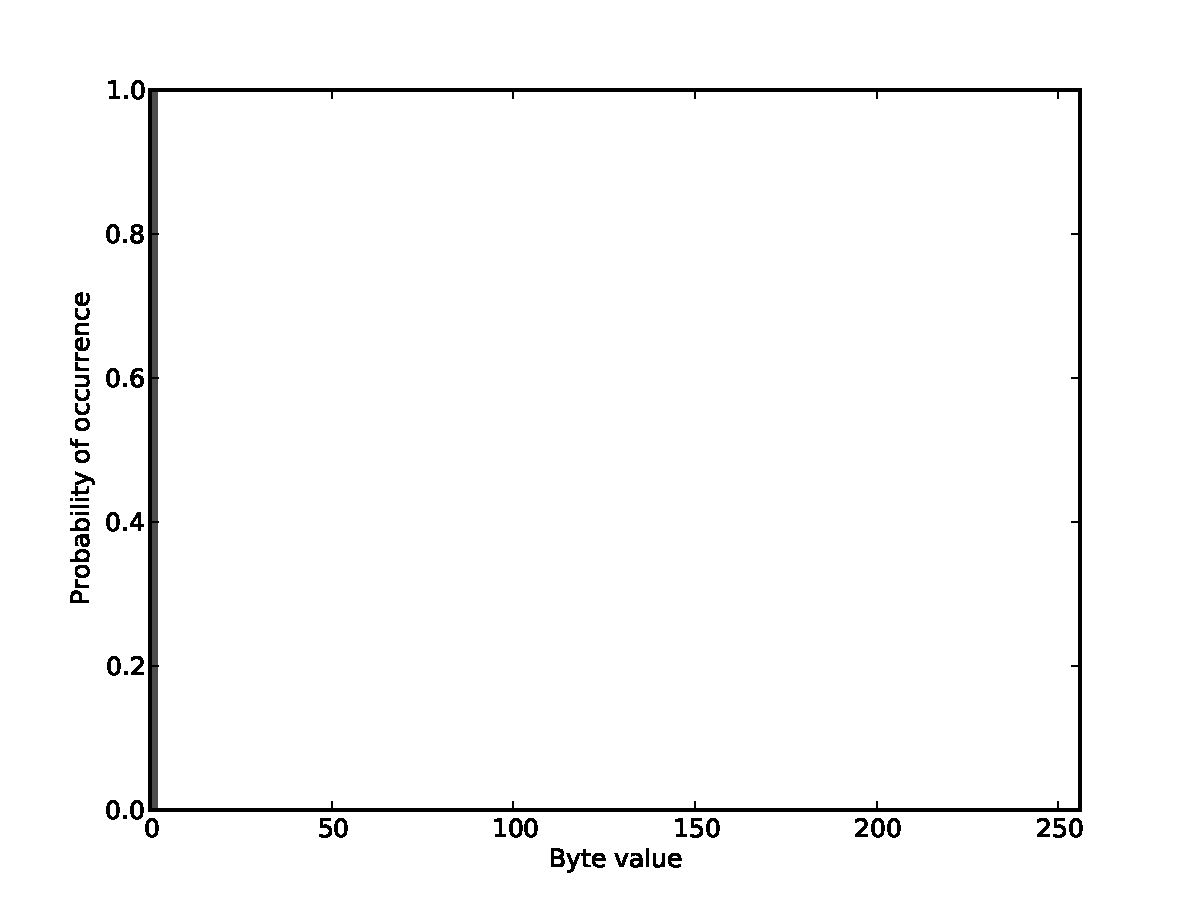
\includegraphics[height=5cm]{img/const_one.pdf}
            \end{column}
        \end{columns}
    \end{frame}
    \begin{frame}
        \frametitle{Flaggfält}
        \begin{columns}[t]
            \begin{column}[T]{6cm}
                Hur vi hittar flaggfält
            \end{column}
            \begin{column}[T]{6cm}
                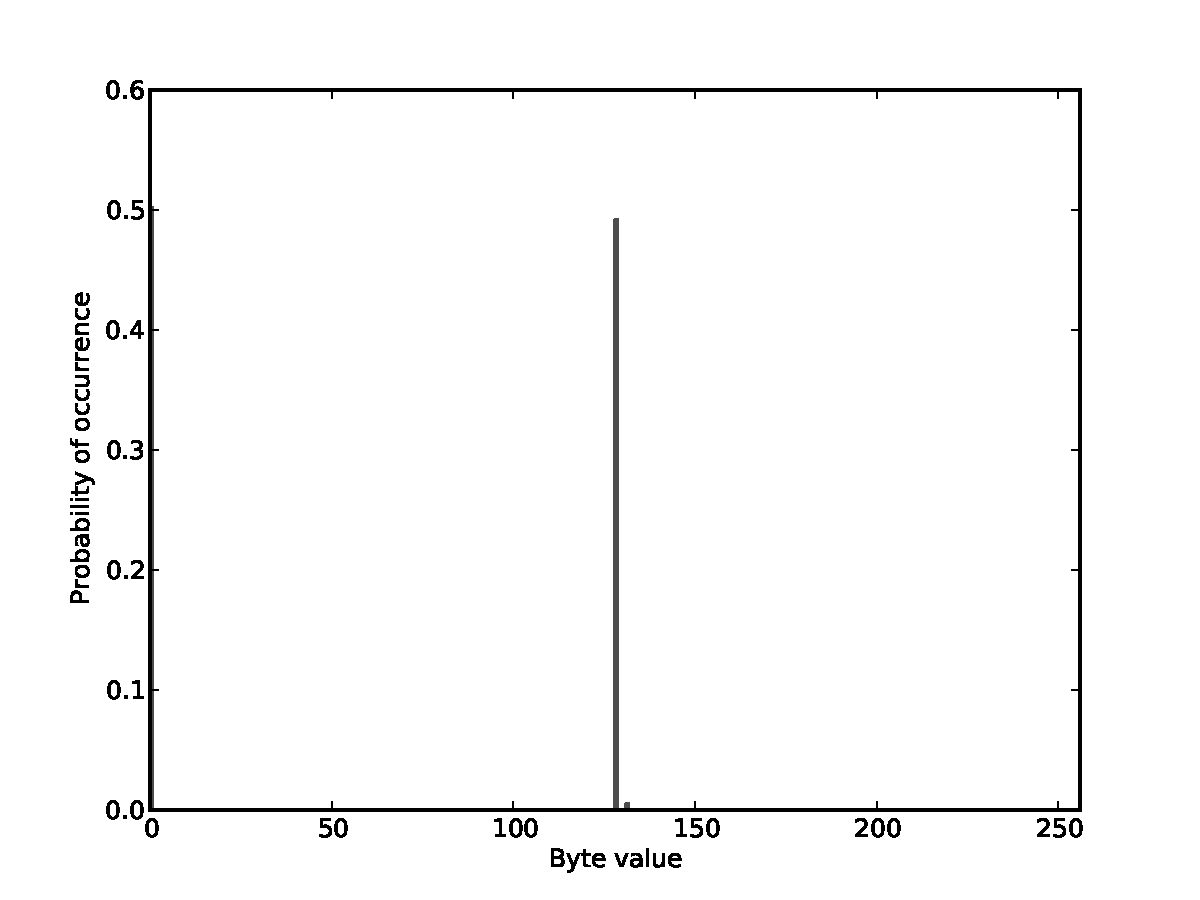
\includegraphics[height=5cm]{img/flag.pdf}
            \end{column}
        \end{columns}
    \end{frame}
    \begin{frame}
        \frametitle{Uniformt fördelade fält}
        \begin{columns}[t]
            \begin{column}[T]{6cm}
                Hur vi hittar uniformt fördelade fält
            \end{column}
            \begin{column}[T]{6cm}
                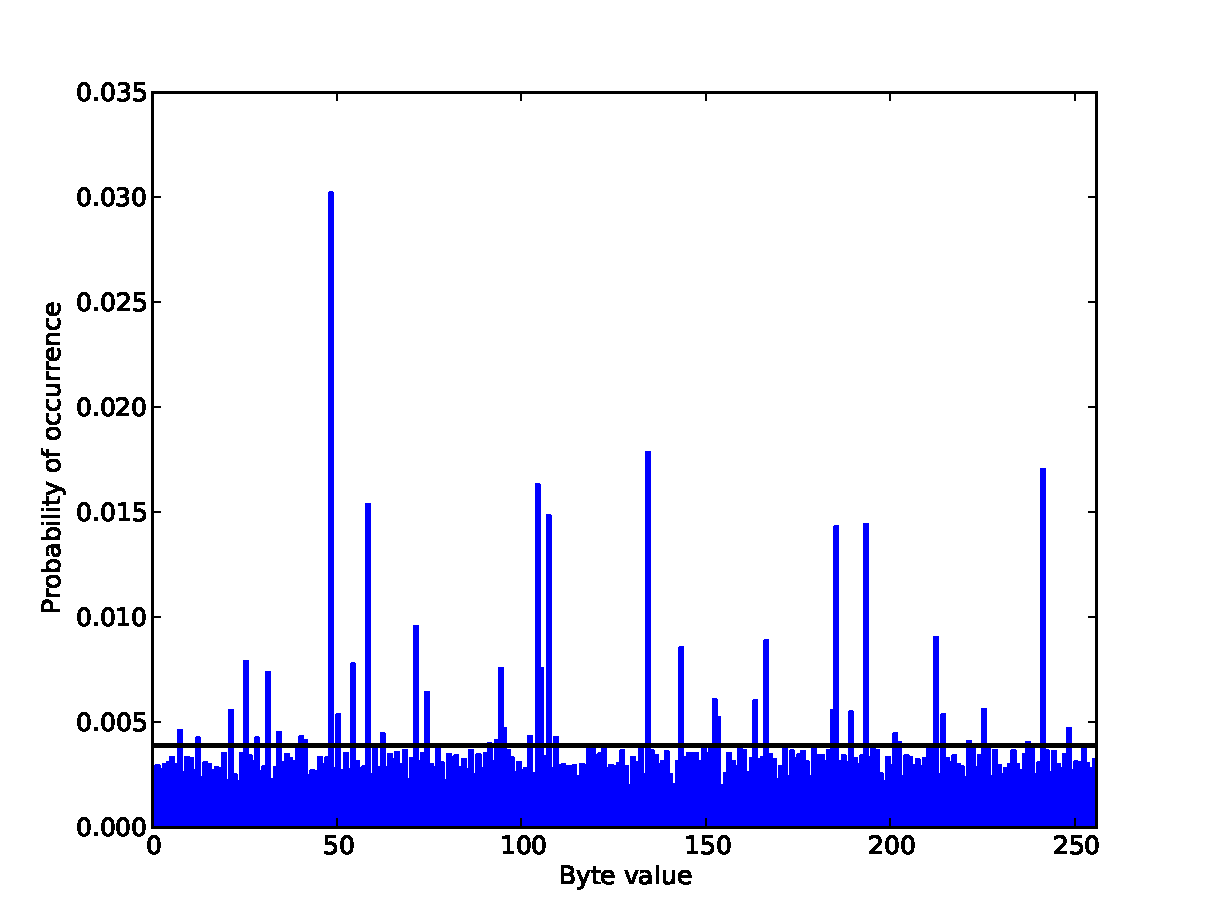
\includegraphics[height=5cm]{img/uniform.pdf}
            \end{column}
        \end{columns}
    \end{frame}
    \begin{frame}
        \frametitle{Nummerfält}
        \begin{columns}[t]
            \begin{column}[T]{6cm}
                Hur vi hittar nummerfält
            \end{column}
            \begin{column}[T]{6cm}
                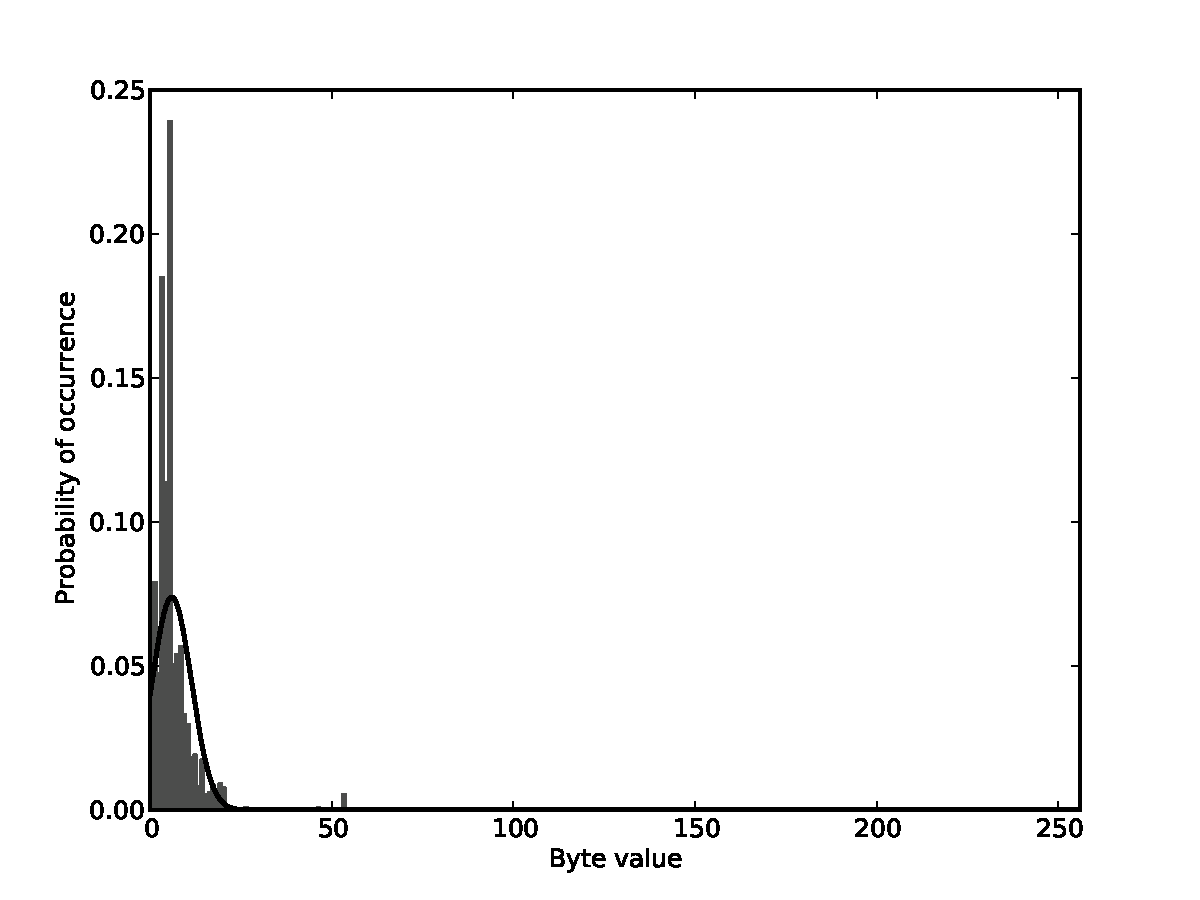
\includegraphics[height=5cm]{img/number.pdf}
            \end{column}
        \end{columns}
    \end{frame}
    \begin{frame}
        \frametitle{Inkrementella fält}
        Hur vi hittar inkrementella fält
    \end{frame}
    \begin{frame}
        \frametitle{Längdfält}
        \begin{columns}[t]
            \begin{column}[T]{6cm}
                Hur vi hittar längdfält
            \end{column}
            \begin{column}[T]{6cm}
                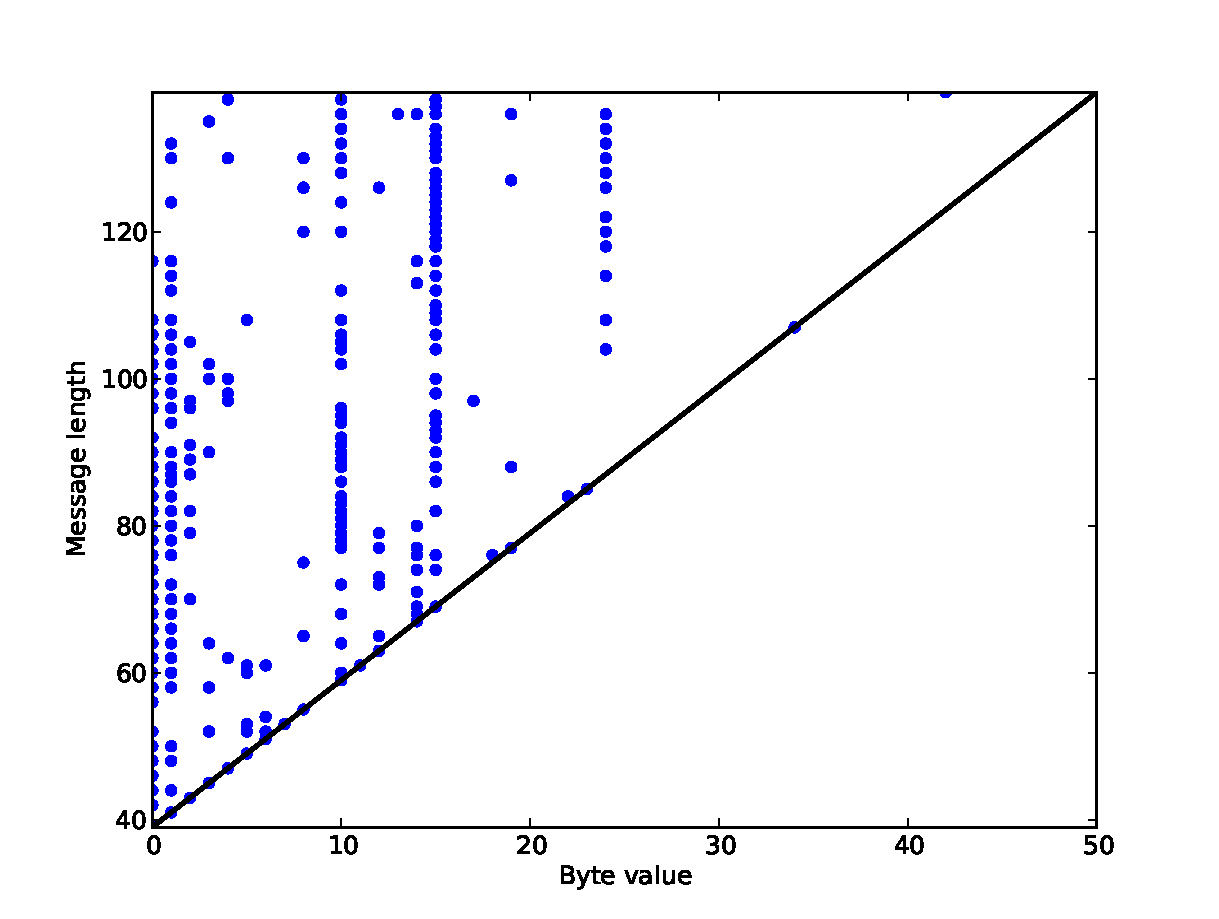
\includegraphics[height=5cm]{img/length.pdf}
            \end{column}
        \end{columns}
    \end{frame}

    % Tillstånd
    \begin{frame}
        \frametitle{Protokolls tillstånd}
        Beskriv hur många protokoll har ett antal tillstånd och hur vi
        hittar dem. Beskriv varför det inte alltid är rimligt att hitta
        alla möjliga tillstånd.
    \end{frame}

    % Resultat
    \begin{frame}
        \frametitle{Resultat}
        Visa resultat och prestanda
    \end{frame}
    \begin{frame}
        \frametitle{Demo?}
        Demonstrera?
    \end{frame}

    % Begränsningar
    \begin{frame}
        \frametitle{Begränsningar}
        Berätta vad som krävs för att kunna göra en bra analys
    \end{frame}

\end{document}
